\documentclass[fleqn]{article}
\usepackage[spanish,es-noshorthands]{babel}
\usepackage[utf8]{inputenc} 
\usepackage[papersize={6.5in,8.5in},total={5.5in,7.25in},centering]{geometry}
\usepackage{mathexam}
\usepackage{amsmath}
\usepackage{graphicx}
\usepackage{multicol}
\usepackage{tikz}

\ExamClass{
\includegraphics[height=16pt]{Images/logo-sed.png} Matemáticas $11^{\circ}$}
\ExamName{``Evaluación 2''}
\ExamHead{
\includegraphics[height=16pt]{Images/logo-colegio.png} IEDAB}
\newcommand{\LineaNombre}{%
\par
\vspace{\baselineskip}
Nombre:\hrulefill \; Curso: \underline{\hspace*{48pt}} \; Fecha: \underline{\hspace*{2.5cm}} \relax
\par}
\let\ds\displaystyle

\begin{document}
\ExamInstrBox{
Respuesta sin justificar mediante procedimiento no será tenida en cuenta en la calificación. Escriba sus respuestas en el espacio indicado o en una hoja anexa y las últimas 5, en el cuadro de respuestas que está al final. Tiene 45 minutos para contestar esta prueba.}
\LineaNombre
\begin{enumerate}
 \item Halle la distancia entre los números $-3$ y 8 usando como herramienta el valor absoluto y determine el punto medio.\noanswer
 \item Ubique en un plano cartesiano los puntos $A(-2,-3)$, $B(4,5)$, $C(-4,2)$ y $D(3,-5)$ y halle la distancia $\overline{AB}$
  \item Sabiendo que la ecuación estandard de la circunferencia de radio $r$, centrada en el punto $(h,k)$ es $(x-h)^{2}+(y-k)^{2}=r^{2}$, determine la ecuación standard de la circunferencia cuyo centro es el punto $(-2,3)$ y de radio $r=3$ \noanswer
 \item Teniendo en cuenta el siguiente gráfico
 \begin{center}
 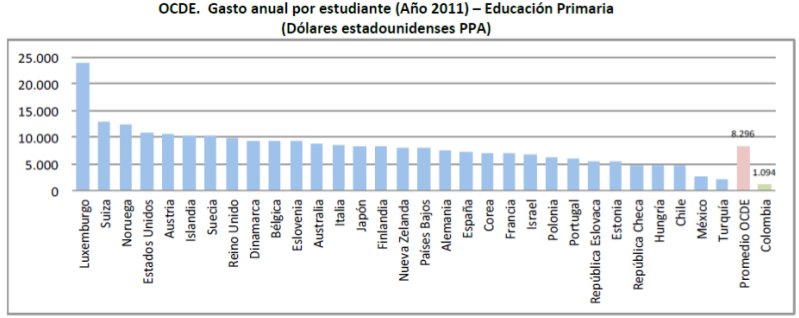
\includegraphics[scale=.45]{Images/GastoEstudEducPrim.png} 
 \end{center}
 Conteste.
 \begin{enumerate}
 \item Si el dolar está a \$2\,865 (pesos), ¿Cuántos pesos colombianos gastaba el gobierno colombiano en un estudiante de primaria al año en el 2011? ¿Cuánto gastaba en promedio un país de la OCDE?
 \newpage
 \item Estime en pesos, el gasto por estudiante al año en Luxemburgo en el 2011 \noanswer
 \item En pesos colombianos, ¿cuál es la diferencia de inversión entre el promedio de los países de la OCDE y Colombia?\noanswer
 \item Cree Ud que con el nivel de inversión por estudiante en Colombia, (que no difiere mucho de la inversión actual) podrá Colombia ser el país mas educado de América Latina, como dice el \emph{slogan} del gobierno?\noanswer
 \end{enumerate}
 \item Construya las primeras 7 filas del triángulo de Pascal. Con base en éste, calcule \noanswer
 \begin{enumerate}
 \begin{multicols}{3}
 \item $\displaystyle{6 \choose 3}$
 \item $\displaystyle{6 \choose 4}$
 \item $\displaystyle{6 \choose 5}$
 \end{multicols}
 \end{enumerate}
 \item ¿Cuál de las siguientes opciones es el punto medio del segmento de recta con extremos $-3$ y 2? Justifique su respuesta
 \begin{enumerate}
 \begin{multicols}{5}
 \item $5/2$
 \item 1
 \item $-1/2$
 \item $-1$
 \item $-5/2$
 \end{multicols}
 \end{enumerate}
 \item ¿Cuál de las siguientes opciones es el centro de la circunferencia $(x - 3)^{2}+ (y+4)^{2}=2$?
 \begin{enumerate}
 \begin{multicols}{5}
 \item $(3,-4)$
 \item $(-3,4)$
 \item $(4,3)$
 \item $(-4,3)$
 \item $(3/2,-2)$
 \end{multicols}
 \end{enumerate}
 \item ¿Cuál de los puntos siguientes está en el tercer cuadrante?
 \begin{enumerate}
 \begin{multicols}{5}
 \item $(0,-3)$
 \item $(-1,0)$
 \item $(2,1)$
 \item $(-1,2)$
 \item $(-2,-3)$
 \end{multicols}
 \end{enumerate}
 \item ¿Cuál de los siguiente números no aparece en el décimo renglón del triángulo de Pascal
 \begin{enumerate}
 \begin{multicols}{5}
 \item 1
 \item 5
 \item 10
 \item 120
 \item 252
 \end{multicols}
 \end{enumerate}
 \item $(x+y)^{3}-(x-y)^{3}=$
 \begin{enumerate}
 \begin{multicols}{5}
 \item 0
 \item $2x^{3}$
 \item $2x^{3}-2y^{3}$
 \item $2x^{3}+6xy^{2}$
 \item $6xy^{2}+2y^{3}$
 \end{multicols}
 \end{enumerate}
 \end{enumerate}
 \begin{center}
\begin{tabular}{cccccccccccc}
6 & 7 & 8 & 9 & 10 \\ 
\textcircled{a} & \textcircled{a} & \textcircled{a} & \textcircled{a} & \textcircled{a}\\ 
\textcircled{b} & \textcircled{b} & \textcircled{b} & \textcircled{b} & \textcircled{b} \\ 
\textcircled{c} & \textcircled{c} & \textcircled{c} & \textcircled{c} & \textcircled{c}\\ 
\textcircled{d} & \textcircled{d} & \textcircled{d} & \textcircled{d} & \textcircled{d} \\ 
\end{tabular} 
\end{center}
\end{document}
